\chapter{Event Selection}
\label{chapter:event_selection}

This chapter defines the signal regions (SRs) targeting the processes shown in Figure~\ref{fig:u1_taunu_target_topologies}.
The analysis variables and preselection are introduced first, followed by the optimisation of the one-$b$-jet regions, the definition of the zero-$b$-jet regions, and a study of $\tau\tau$ signal contamination in the SRs.

\section{Preselection and variables definition}
\label{sec:ch7_preselection}

\subsection{Analysis variables}
\label{subsec:ch7_variables}

The transverse mass $\mT$ of the $\tau$ and $\mpt$ system is defined as
    \begin{equation}
        \mT = \sqrt{2\pT^\tau\met\left[1-\cos\DphiTauMet\right]}.
        \label{eq:ch7_mt}
    \end{equation}
Here $\DphiTauMet$ is the separation in $\phi$ between the $\tau$ momentum and $\mpt$.
The variable $\mT$ is used to probe the high-energy tail of the $\tau\nu$ final state, which is particularly sensitive to non-resonant leptoquark contributions~\cite{Endo2022NonResonant}.

The invariant masses $m_{b\tau}$ and $m_{j\tau}$ are defined as:
    \begin{equation}
        m_{b\tau}^{2} = (p_b+p_\tau)^2, \qquad m_{j\tau}^{2} = (p_{j_1}+p_\tau)^2,
        \label{eq:ch7_visible_masses}
    \end{equation}
    where $p_b$, $p_{j_1}$ and $p_\tau$ are four-momenta, and $j_1$ is the jet with the largest $\pT$.
The zero-$b$-jet regions contain no $b$-tagged jet, so $m_{j\tau}$ is used in place of $m_{b\tau}$.

\subsection{Multijet suppression and Preselection}
\label{subsec:ch7_multijet}

Multijet events can enter the SR and CR selections due to the misidentified $\tau$ and $\met$ due to the poor jet resolution.
Although a high $\met$ threshold rejects most of these events, further suppression is necessary due to their large cross section.
As mentioned above, the high $\met$ is produced when an energetic jet is mismeasured. In this case, the direction of $\mpt$ is approximately towards that jet. Therefore, a small $\Delta\phi$ between the jet and $\mpt$ is expected.
This contribution is referred to as fake $\met$. On the other hand, in signal events, the $\mpt$ from neutrinos has no such tendency.
Figure~\ref{fig:ch7_fake_met} illustrates this difference.

\begin{figure}[htbp]
    \centering
    \begin{subfigure}{0.34\linewidth}
        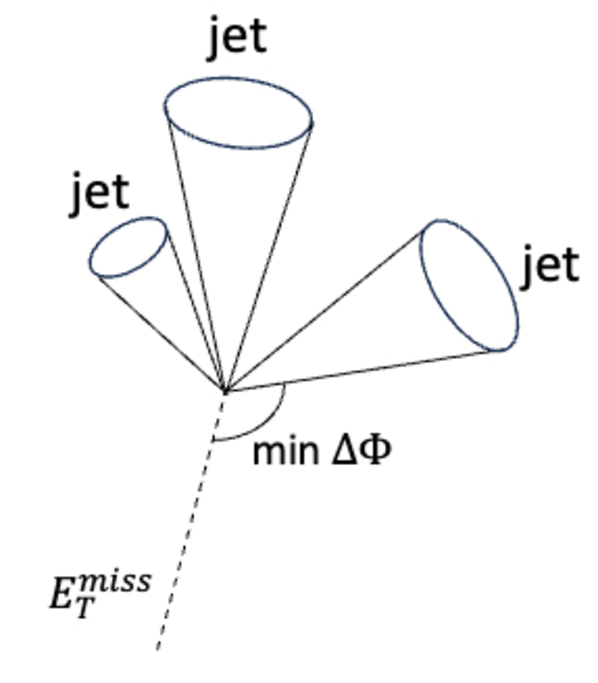
\includegraphics[width=\linewidth]{Figs/CH7/QCD/fake_met_signal.pdf}
        \caption{Signal.}
    \end{subfigure}\hspace{0.08\linewidth}
    \begin{subfigure}{0.34\linewidth}
        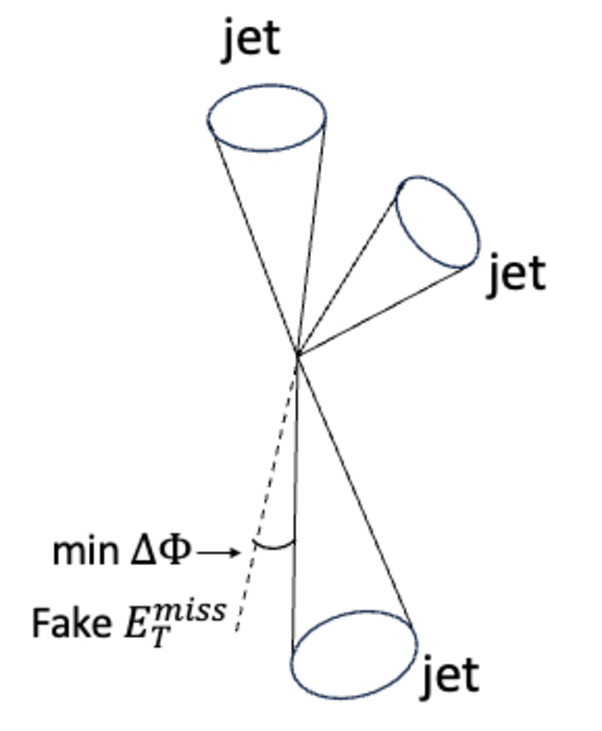
\includegraphics[width=\linewidth]{Figs/CH7/QCD/fake_met_multijets.pdf}
        \caption{Multijet background.}
    \end{subfigure}
    \caption[Missing momentum in signal and multijet events]{Schematic diagrams of (a) $\met$ from neutrinos in signal events and (b) fake $\met$ from a mismeasured energetic jet in multijet events.}
    \label{fig:ch7_fake_met}
\end{figure}

The minimum jet--$\mpt$ separation in $\phi$ and the ratio $\met/\minDphiJetPt$ are used as discriminating variables.
Here $\minDphiJetPt$ is the $\pT$ of the jet with the smallest $\Delta\phi(j,\met)$.
Since fake $\met$ is calculated from a mismeasured jet, multijet events tend to have small $\min\Delta\phi(j,\met)$ and $\met/\minDphiJetPt$.
By contrast, the neutrinos in signal events can produce large $\met$ even when a much softer jet happens to lie nearby in $\phi$.

Events are therefore retained if
\begin{equation}
    \min\Delta\phi(j,\met)>0.4 \quad\text{or}\quad \frac{\met}{\minDphiJetPt}>6.
    \label{eq:ch7_qcd_cut}
\end{equation}
A detailed study is introduced in Appendix~\ref{App:QCD_bkg_study}.

The preselection is applied before the SR optimisation.
Events must pass the lowest-threshold unprescaled $\met$ trigger, requiring $\met>200~\GeV$ for full efficiency.
Exactly one signal $\tau$ and an electron/muon veto are also required, along with the multijet suppression requirement in Eq.~\ref{eq:ch7_qcd_cut}.
For the one b-jet signal region ($\bTagSR$), exactly one $b$-tagged jet is required, while at least one untagged jet is required in $\bVetoSR$.

\section[$\bTagSR$ optimisation and definition]{$\bTagSR$ optimisation and definition}
\label{sec:ch7_sr1b}

$\bTagSR$ is optimised using the grid scan for variables may help the signal and background seperation. $\bTagSR$-$\Res$ and $\bTagSR$-$\NonRes$ are optimised seperatedly. %需要优化下英语表达

\subsection{Scan variables and optimisation criterion}
\label{subsec:ch7_scan}

$\pT^\tau$ and $\met$ are selected in the first place as the signiture tend to have energetic $\tau$ leptons and neutrinos.
$b$-jet $\pT$ is also selected, with the consider of $\NonRes$ 

High values of $\mT$ are selected to distinguish non-resonant leptoquark exchange from the falling SM background.
A tighter $\mT$ threshold is therefore imposed in $\bTagSR$-$\NonRes$ than in $\bTagSR$-$\Res$, where the $b\tau$ mass is also used.

The invariant mass $m_{b\tau}$ is used to probe resonant $U_1\to b\tau$ decays, while the SM backgrounds have no corresponding heavy resonance.
The signal distribution is shifted below $\MU$ and broadened by the $\tau$-decay neutrino, with additional smearing from the jet and $\tau$ energy resolutions.
A lower mass threshold is imposed to suppress the SM backgrounds while retaining this broad signal.

The separation $\DphiTauMet$ is used to select the approximately back-to-back $\tau$ and $\mpt$ configuration of the non-resonant signal, which helps suppress top-quark backgrounds.
Resonant leptoquark production is also suppressed by a strong back-to-back requirement, because the transverse momentum balance is modified by the decay jet.

The jet multiplicity $N_j-N_b$ tends to be larger in $\ttbar$ events because the two top-quark decays produce additional jets.
An upper limit is imposed to suppress this background while retaining signal events with fewer jets.

The kinematic thresholds are scanned together because the discriminating variables are correlated.
For example, increasing $\met$ also raises $\mT$ at fixed $\pT^\tau$ and $\DphiTauMet$, so the effect of an additional $\mT$ requirement depends on the other cuts.

Lower thresholds on $\pT^\tau$, $\met$ and $\mT$ are scanned in both $\bTagSR$ regions, together with an upper limit on $N_j-N_b$.
A lower threshold on $\DphiTauMet$ is tested for the non-resonant topology.
For the resonant topology, upper thresholds on this angle and a lower threshold on $m_{b\tau}$ are tested, as summarised in Table~\ref{tab:ch7_scan_variables}.

\begin{table}[htbp]
    \centering
    \small
    \caption{Thresholds tested in the $\bTagSR$ optimisation. Each set lists the trial values for the indicated inequality. A zero mass threshold or an angular upper threshold of $\pi$ represents no effective requirement on that variable.}
    \label{tab:ch7_scan_variables}
    \begin{tabular}{lcc}
        \toprule
        Variable & $\bTagSR$-$\Res$ & $\bTagSR$-$\NonRes$ \\
        \midrule
        $\DphiTauMet$ & $<\{0.3,1.2,2.4,2.6,\pi\}$ & $>\{0.3,1.2,2.4,2.6\}$ \\
        $m_{b\tau}$ [$\GeV$] & $>\{0,800\}$ & Not scanned \\
        $\met$ [$\GeV$] & \multicolumn{2}{c}{$>\{200,250,300,350,400,500,600\}$} \\
        $\pT^\tau$ [$\GeV$] & \multicolumn{2}{c}{$>\{200,250,300,350,400,500,600\}$} \\
        $\mT$ [$\GeV$] & \multicolumn{2}{c}{$>\{100,200,300,400,500,600,700,800,900,1000\}$} \\
        $N_j-N_b$ & \multicolumn{2}{c}{$\leq\{1,2,3\}$} \\
        \bottomrule
    \end{tabular}
\end{table}

The mass scan uses only $m_{b\tau}>0$ and $800~\GeV$.
The broad $m_{b\tau}$ distribution and limited simulated background statistics in its high-mass tail favour an inclusive mass requirement over a finely scanned mass window.

The resonant optimisation targets $\MU=1.5~\TeV$, where on-shell production is important.
The non-resonant optimisation uses $(\MU,\gU,\beta_L^{23})=(2.5~\TeV,2.5,1.0)$, where virtual exchange provides the dominant signal contribution.

The expected sensitivity of each cut combination is ranked using an approximate counting-experiment significance~\cite{ATL-PHYS-PUB-2020-025}:
\begin{equation}
    Z = \sqrt{2\left[n\ln\!\left(\frac{n(b+\sigma_b^2)}{b^2+n\sigma_b^2}\right)-\frac{b^2}{\sigma_b^2}\ln\!\left(\frac{b^2+n\sigma_b^2}{b(b+\sigma_b^2)}\right)\right]},
    \label{eq:ch7_optimisation_significance}
\end{equation}
where $s$ and $b$ are the expected signal and background event yields, $n=s+b$, and $\sigma_b$ is the absolute uncertainty in the background expectation.
A fractional background uncertainty of $30\%$, corresponding to $\sigma_b=0.30b$, is assumed for this scan.
The scan uses the pure BSM signal yield.
The effect of interference on the final signal prediction is discussed below.
The quantity $Z$ is used to compare selections, while the final confidence limits are obtained with the likelihood analysis in Chapter~\ref{chapter:results}.

Cut combinations with $b\leq2$ are discarded to avoid selecting apparently background-free regions caused by limited MC statistics.
If a particular simulated background has a negative weighted yield after a trial selection, its contribution is set to zero when evaluating the scan criterion.
This is a prescription for comparing trial cuts in sparse simulated samples.
It does not imply a negative physical event rate.

\subsection{Interference and signal efficiency}
\label{subsec:ch7_efficiency}

The interference term in Eq.~\ref{eq:signal_interference} changes the signal contribution remaining after the selection.
If $S$ denotes the pure BSM yield and $I$ the interference yield, the excess above the SM prediction is $S+I$ at the nominal signal normalisation.
Destructive interference gives $I<0$, so a selection ranked using $S$ alone can overestimate the final sensitivity.
Its effect is therefore checked after the optimisation and included in the final statistical model.

The requirements on $\pT^\tau$, $\met$ and $\mT$ suppress the low-energy phase space in which interference with SM $W$ production is most important.
In particular, the non-resonant requirements $\pT^\tau>200~\GeV$, $\met>400~\GeV$ and $\mT>600~\GeV$ retain the hard tail while reducing the destructive contribution.
The residual interference has a negligible effect on the sensitivity of the one-$b$-jet regions in the parameter range probed by the analysis.
This conclusion does not apply to the zero-$b$-jet regions, where the interference contribution must be retained, as discussed in Section~\ref{sec:ch7_sr0b}.

The signal efficiency is monitored through the cumulative cutflow in Table~\ref{tab:ch7_cutflow}.
For $(\MU,\gU,\beta_L^{23})=(1.5~\TeV,1.5,0.6)$, the resonant selection retains 4.2 of the 35.2 expected signal events passing the one-$b$-jet baseline, or approximately $12\%$.
For the non-resonant optimisation benchmark, it retains 6.6 of 111.0 events, or approximately $6\%$.
The background decreases from approximately 4027 baseline events to 2.4 and 2.1 events, respectively.
These fractions describe signal retention during the cut optimisation and use the baseline sample as their denominator.
The acceptance times selection efficiency, $A\epsilon$, instead uses the total generated signal as its reference and includes the kinematic acceptance and reconstruction and selection losses.
The cutflow uses the pure BSM contribution because the signed interference yield is not an event-selection efficiency.
The tabulated numbers describe the optimisation study before the background fit, while the final selections are chosen with the statistical uncertainty in the background prediction kept below $30\%$.

\begin{table}[htbp]
    \centering
    \small
    \caption{Cumulative signal ($S$) and background ($B$) yields in the one-$b$-jet optimisation. The resonant and non-resonant signal benchmarks are $(\MU~[\TeV],\gU,\beta_L^{23})=(1.5,1.5,0.6)$ and $(2.5,2.5,1.0)$, respectively. These are simulated expectations before the background fit.}
    \label{tab:ch7_cutflow}
    \begin{tabular}{lrrlrr}
        \toprule
        \multicolumn{3}{c}{Resonant} & \multicolumn{3}{c}{Non-resonant} \\
        Cumulative requirement & $S$ & $B$ & Cumulative requirement & $S$ & $B$ \\
        \midrule
        Baseline & 35.2 & 4027.3 & Baseline & 111.0 & 4027.3 \\
        $\pT^\tau>200~\GeV$ & 19.9 & 193.1 & $\pT^\tau>200~\GeV$ & 70.5 & 193.1 \\
        $\met>200~\GeV$ & 19.9 & 193.1 & $\met>400~\GeV$ & 26.4 & 15.1 \\
        $\mT>200~\GeV$ & 19.4 & 143.6 & $\mT>600~\GeV$ & 24.0 & 6.4 \\
        $m_{b\tau}>800~\GeV$ & 4.9 & 5.2 & $\DphiTauMet>1.2$ & 23.8 & 6.4 \\
        $N_j-N_b\leq3$ & 4.7 & 4.3 & $N_j-N_b\leq1$ & 17.2 & 2.8 \\
        $\pT^b>250~\GeV$ & 4.2 & 2.4 & $50<\pT^b<250~\GeV$ & 6.6 & 2.1 \\
        \bottomrule
    \end{tabular}
\end{table}

\subsection{Selected regions and background composition}

The selected $\bTagSR$-$\Res$ requirements are $\pT^\tau>200~\GeV$, $\met>200~\GeV$, $\mT>200~\GeV$ and $m_{b\tau}>800~\GeV$, with at most three jets that are not $b$-tagged.
No additional $\DphiTauMet$ requirement is retained.
The region is treated as a single event-counting bin because the available background simulation does not support a finely binned fit to the broad $m_{b\tau}$ distribution.

The selected $\bTagSR$-$\NonRes$ requirements are $\pT^\tau>200~\GeV$, $\met>400~\GeV$, $\mT>600~\GeV$ and $\DphiTauMet>1.2$, with at most one jet that is not $b$-tagged.
No $m_{b\tau}$ requirement is imposed because the $b$-jet and $\tau$ do not reconstruct an on-shell leptoquark in the target topology.
This region also contributes a single event count to the fit.

The loose $N-1$ distributions in Figures~\ref{fig:ch7_sr1b_res_distributions} and~\ref{fig:ch7_sr1b_nonres_distributions} illustrate the variables entering the optimisation.
An $N-1$ distribution omits the requirement on the plotted variable while retaining the other requirements.
To make the shapes visible with the available simulation, the resonant $\mT$ and $\pT^\tau$ thresholds are lowered by $100~\GeV$.
For the non-resonant region, the $\mT$, $\met$ and $\pT^\tau$ thresholds are each lowered by $100~\GeV$ before the plotted requirement is removed.
The trigger-plateau requirement $\met>200~\GeV$ is retained.
These distributions therefore illustrate a larger phase space than the final SRs.
The resonant signal has a broad $m_{b\tau}$ distribution, while the non-resonant signal extends into the high-$\mT$ and high-$\met$ tails.

\begin{figure}[p]
    \centering
    \begin{subfigure}{0.49\linewidth}
        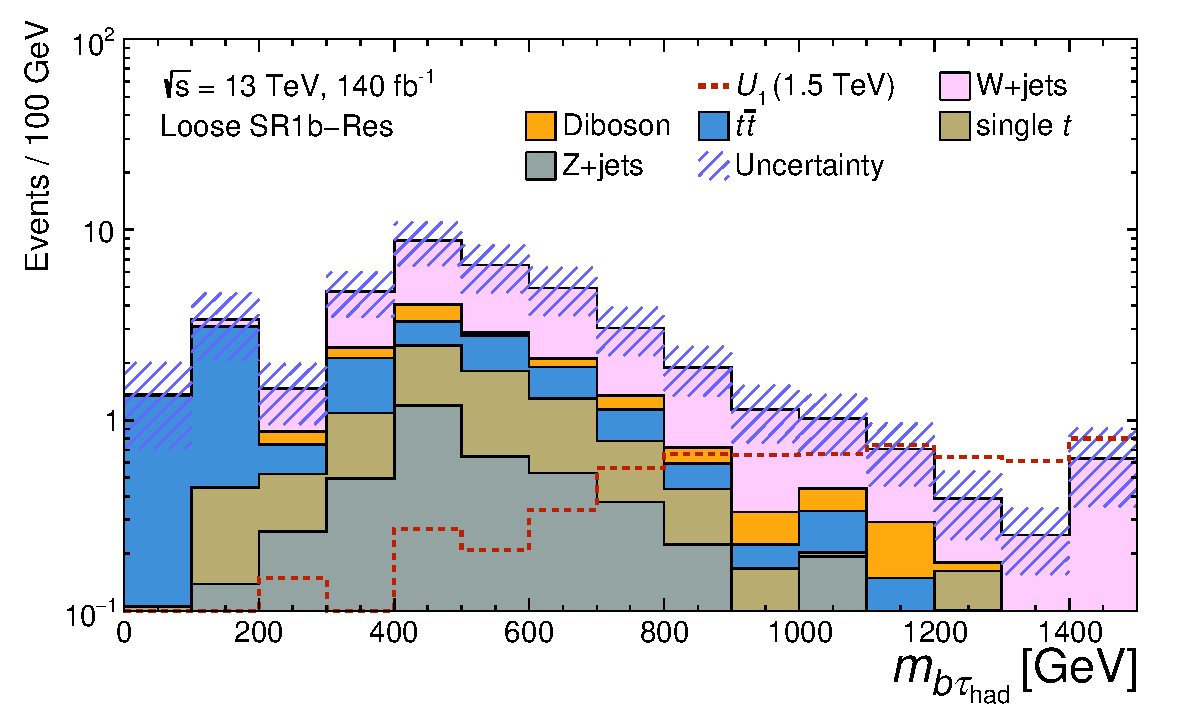
\includegraphics[width=\linewidth]{Figs/CH7/SR1b_Res_InvM.pdf}
        \caption{$m_{b\tau}$.}
    \end{subfigure}\hfill
    \begin{subfigure}{0.49\linewidth}
        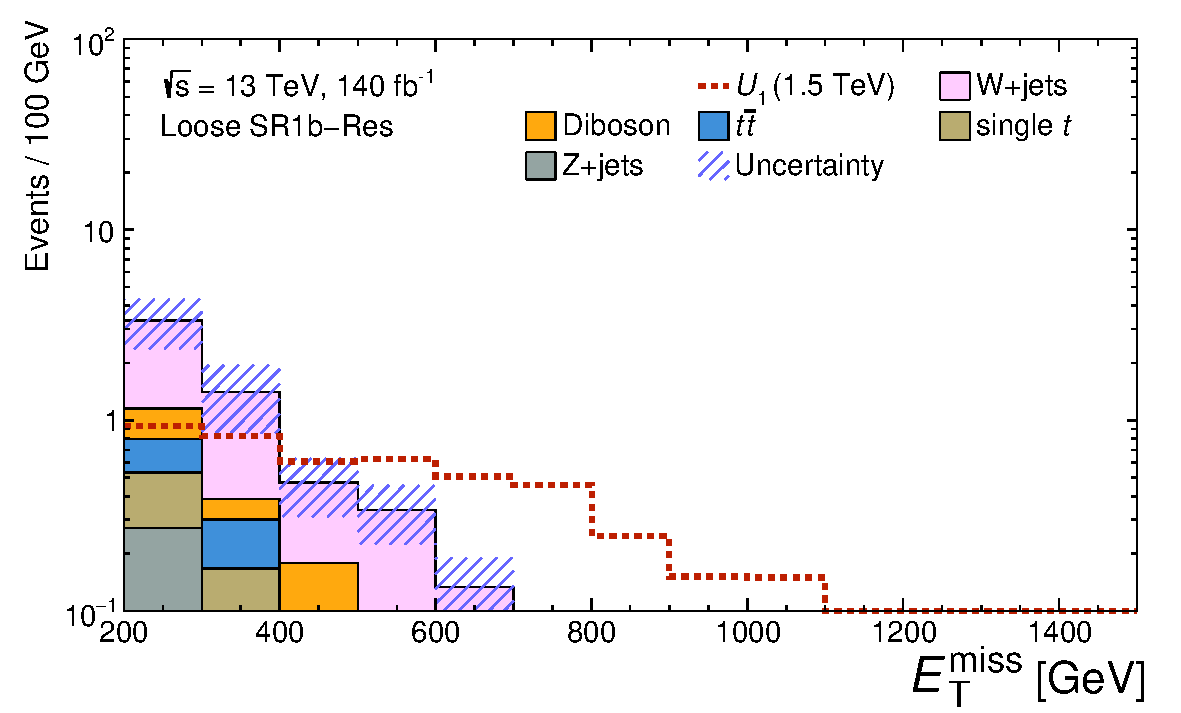
\includegraphics[width=\linewidth]{Figs/CH7/SR1b_Res_met.pdf}
        \caption{$\met$.}
    \end{subfigure}\par\medskip
    \begin{subfigure}{0.49\linewidth}
        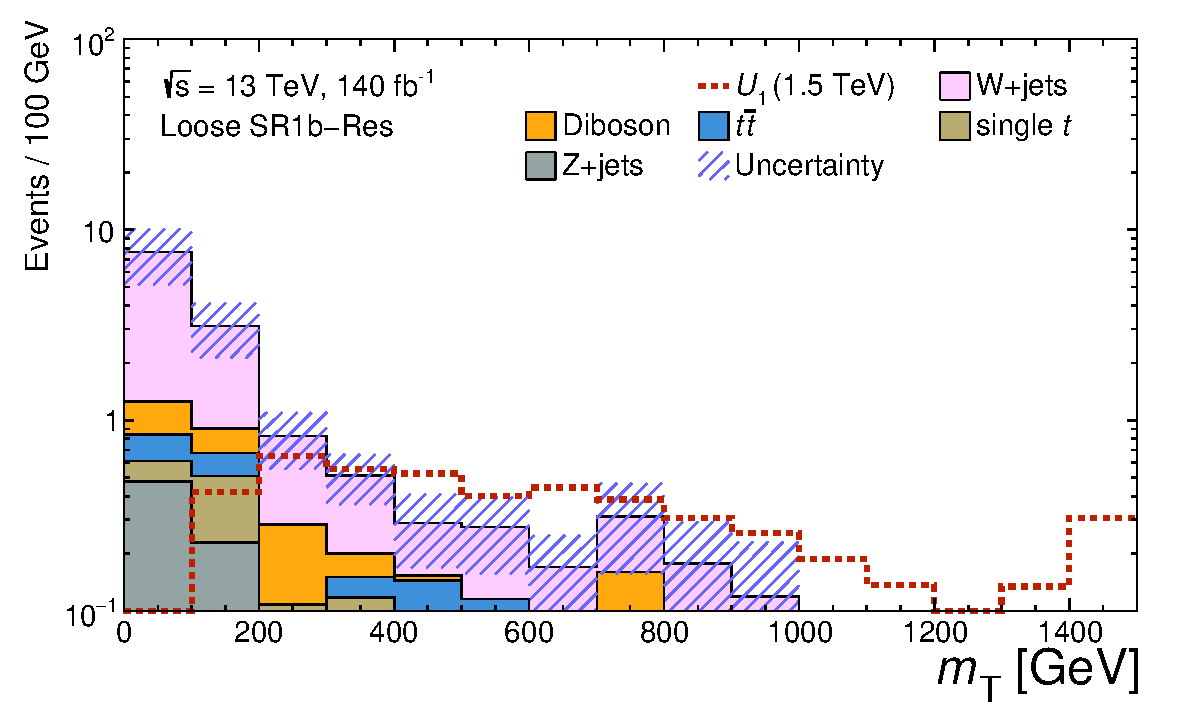
\includegraphics[width=\linewidth]{Figs/CH7/SR1b_Res_mT.pdf}
        \caption{$\mT$.}
    \end{subfigure}\hfill
    \begin{subfigure}{0.49\linewidth}
        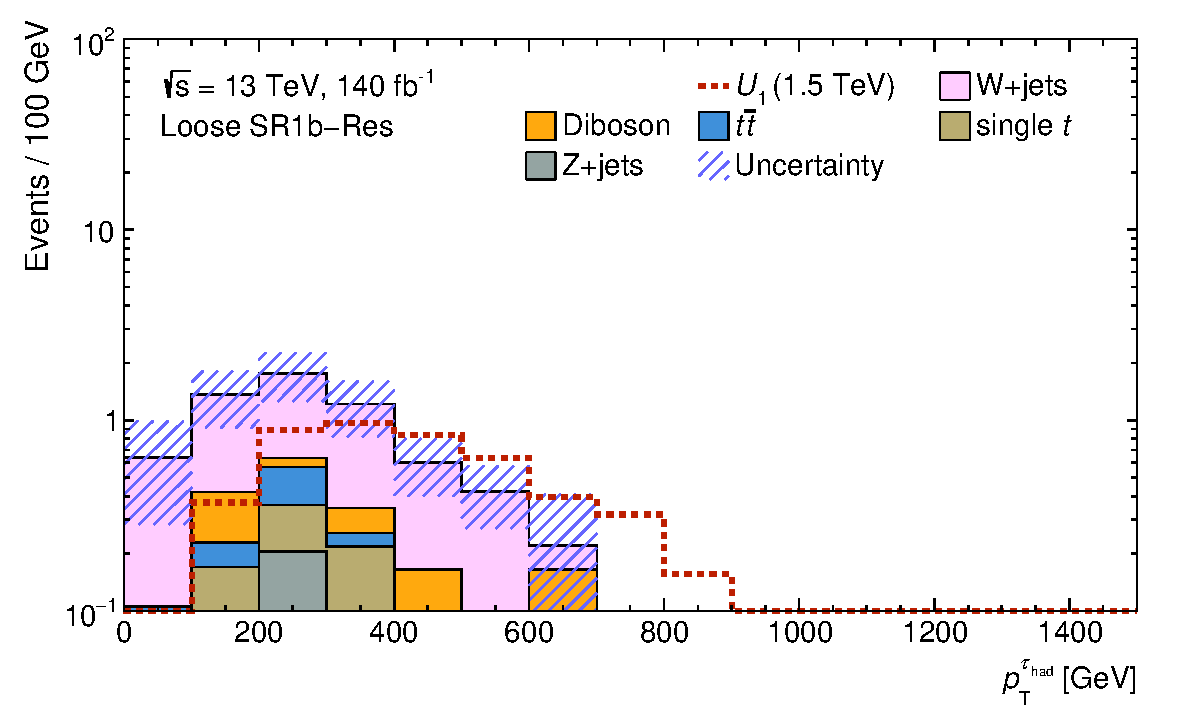
\includegraphics[width=\linewidth]{Figs/CH7/SR1b_Res_tau_pT.pdf}
        \caption{$\pT^\tau$.}
    \end{subfigure}\par\medskip
    \begin{subfigure}{0.49\linewidth}
        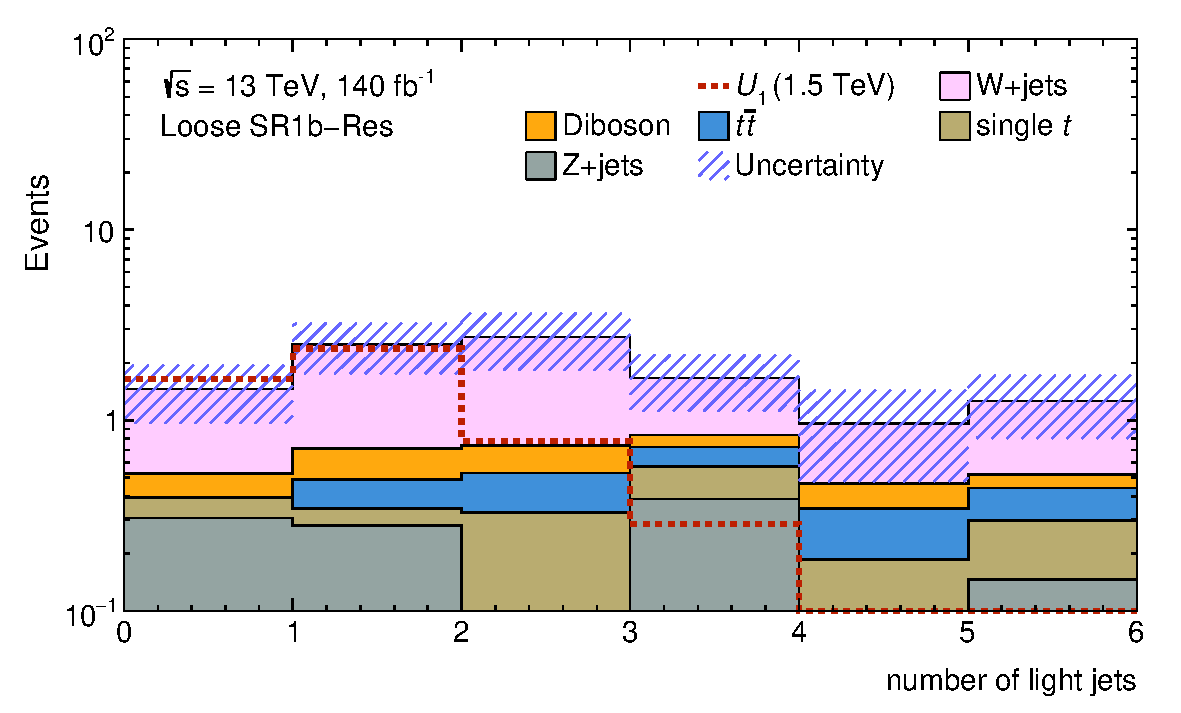
\includegraphics[width=\linewidth]{Figs/CH7/SR1b_Res_nlightjets.pdf}
        \caption{$N_j-N_b$.}
    \end{subfigure}\hfill
    \begin{subfigure}{0.49\linewidth}
        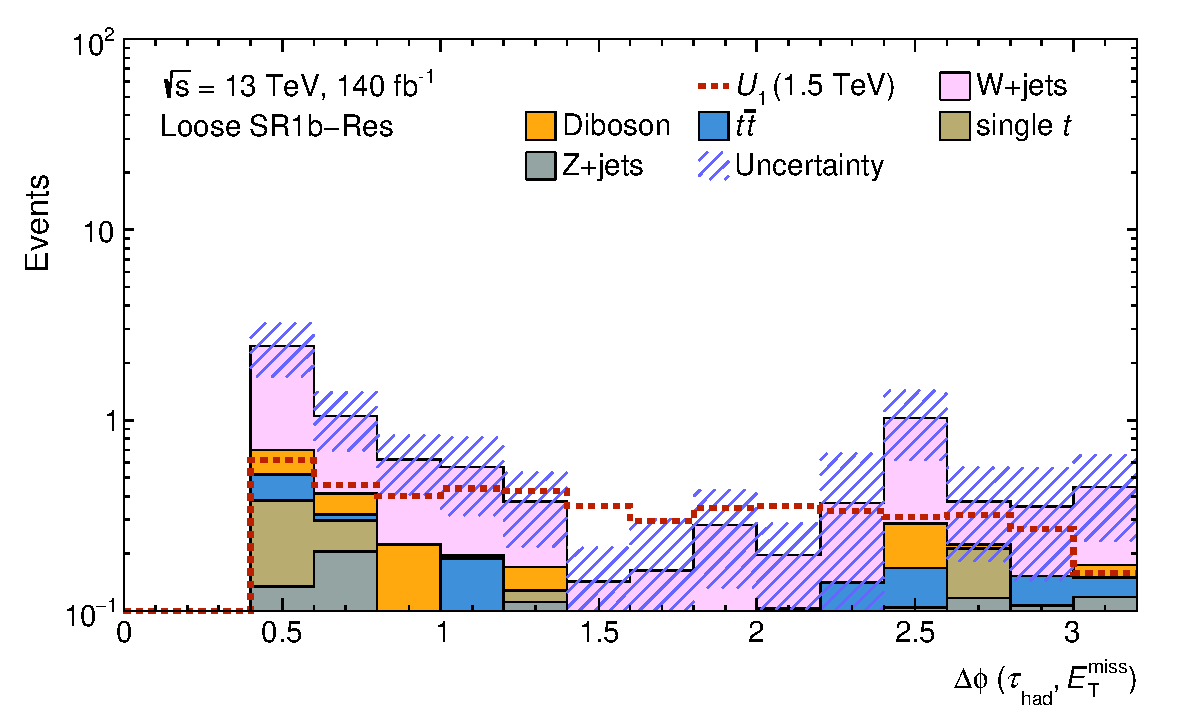
\includegraphics[width=\linewidth]{Figs/CH7/SR1b_Res_dphi.pdf}
        \caption{$\DphiTauMet$.}
    \end{subfigure}\par\medskip
    \caption[Loose N-1 distributions in SR1b-Res]{Distributions of the six scan variables in the loose resonant one-$b$-jet region. The $\mT$ and $\pT^\tau$ thresholds are reduced to $100~\GeV$, and the requirement on each plotted variable is removed, retaining the baseline $\met>200~\GeV$. The stacked backgrounds are shown before the fit. The dotted signal curve is the pure BSM prediction at $(\MU,\gU,\beta_L^{23})=(1.5~\TeV,1.5,0.6)$. The hatched band represents the background uncertainty.}
    \label{fig:ch7_sr1b_res_distributions}
\end{figure}

\begin{figure}[p]
    \centering
    \begin{subfigure}{0.49\linewidth}
        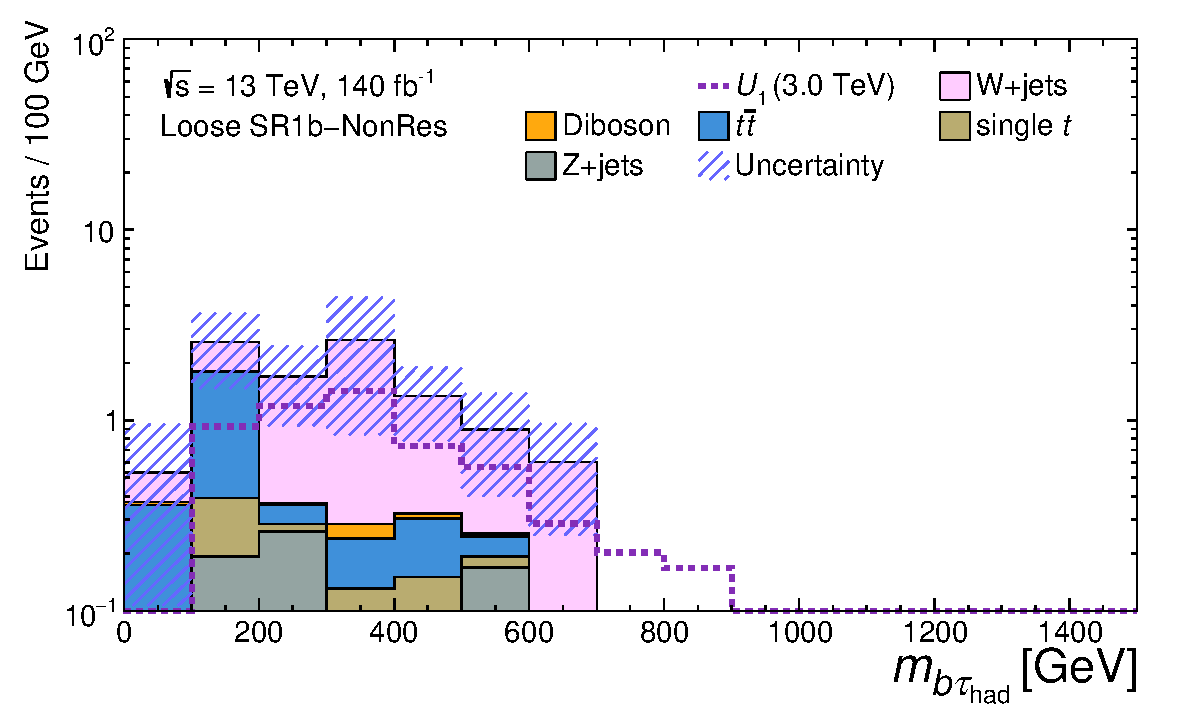
\includegraphics[width=\linewidth]{Figs/CH7/SR1b_NonRes_InvM.pdf}
        \caption{$m_{b\tau}$.}
    \end{subfigure}\hfill
    \begin{subfigure}{0.49\linewidth}
        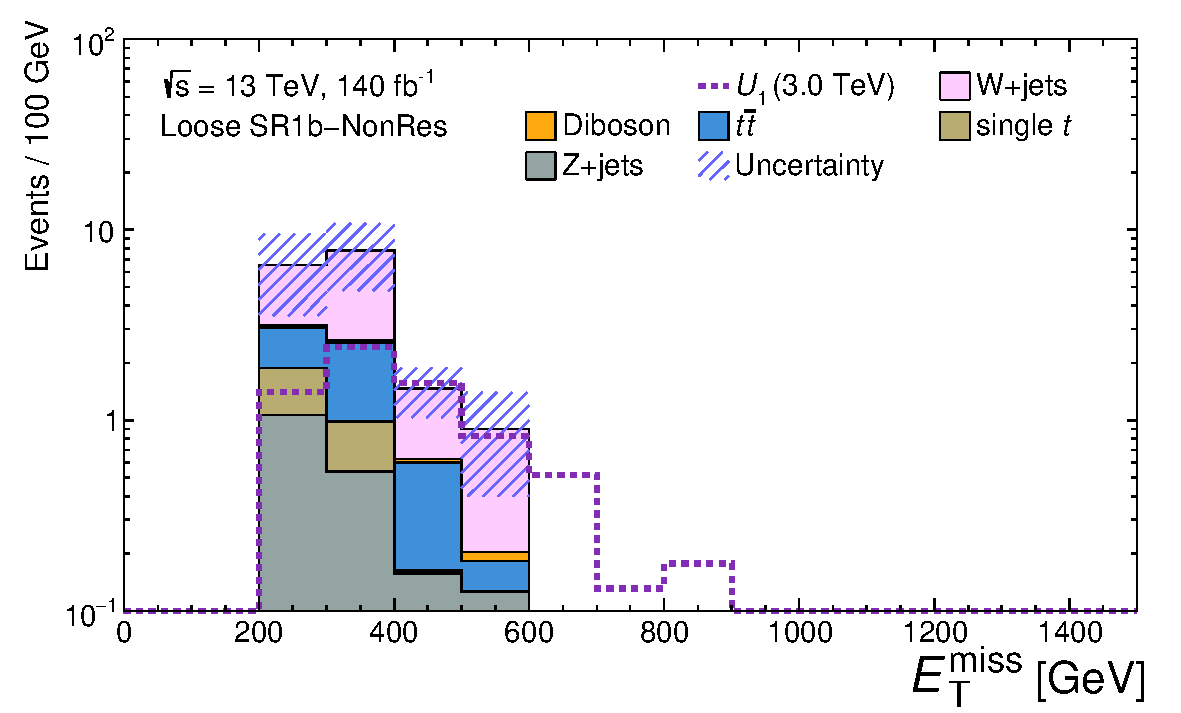
\includegraphics[width=\linewidth]{Figs/CH7/SR1b_NonRes_met.pdf}
        \caption{$\met$.}
    \end{subfigure}\par\medskip
    \begin{subfigure}{0.49\linewidth}
        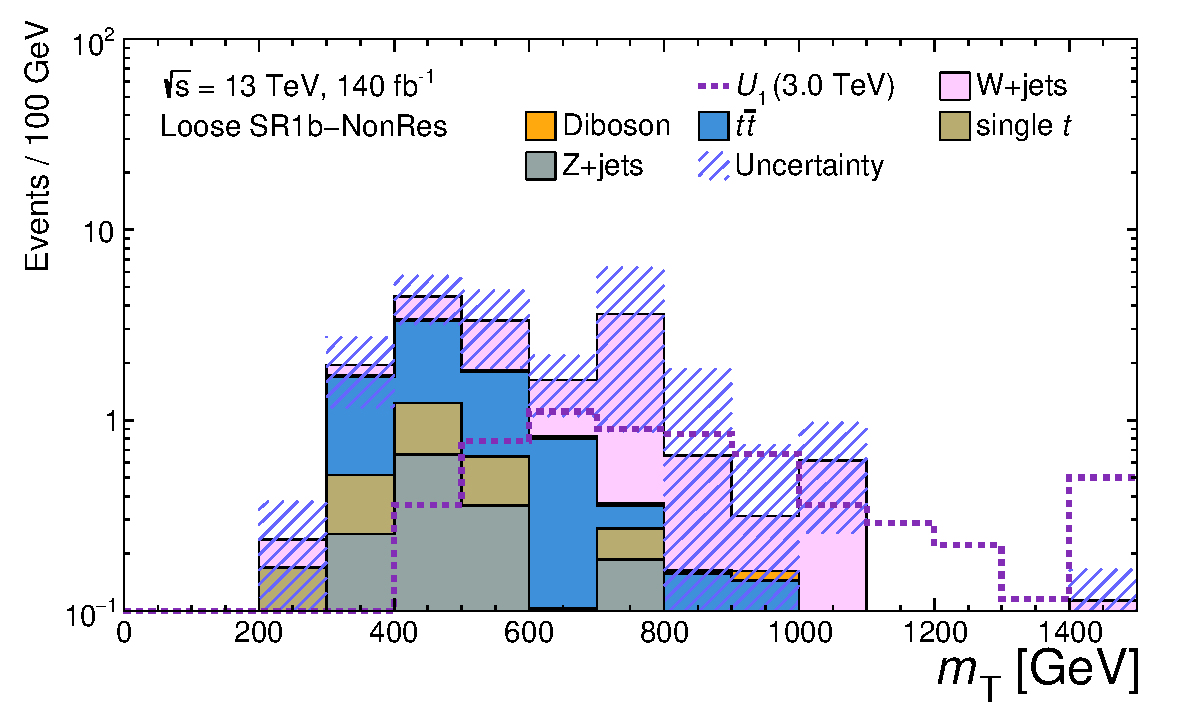
\includegraphics[width=\linewidth]{Figs/CH7/SR1b_NonRes_mT.pdf}
        \caption{$\mT$.}
    \end{subfigure}\hfill
    \begin{subfigure}{0.49\linewidth}
        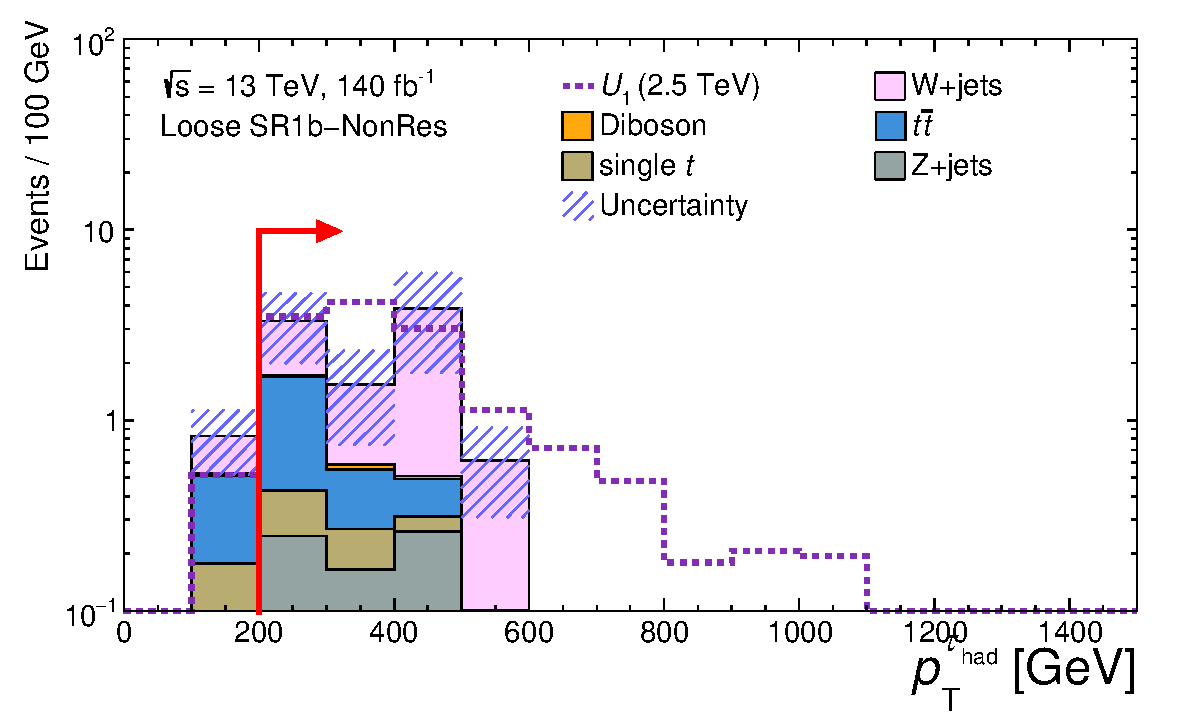
\includegraphics[width=\linewidth]{Figs/CH7/SR1b_NonRes_tau_pT.pdf}
        \caption{$\pT^\tau$.}
    \end{subfigure}\par\medskip
    \begin{subfigure}{0.49\linewidth}
        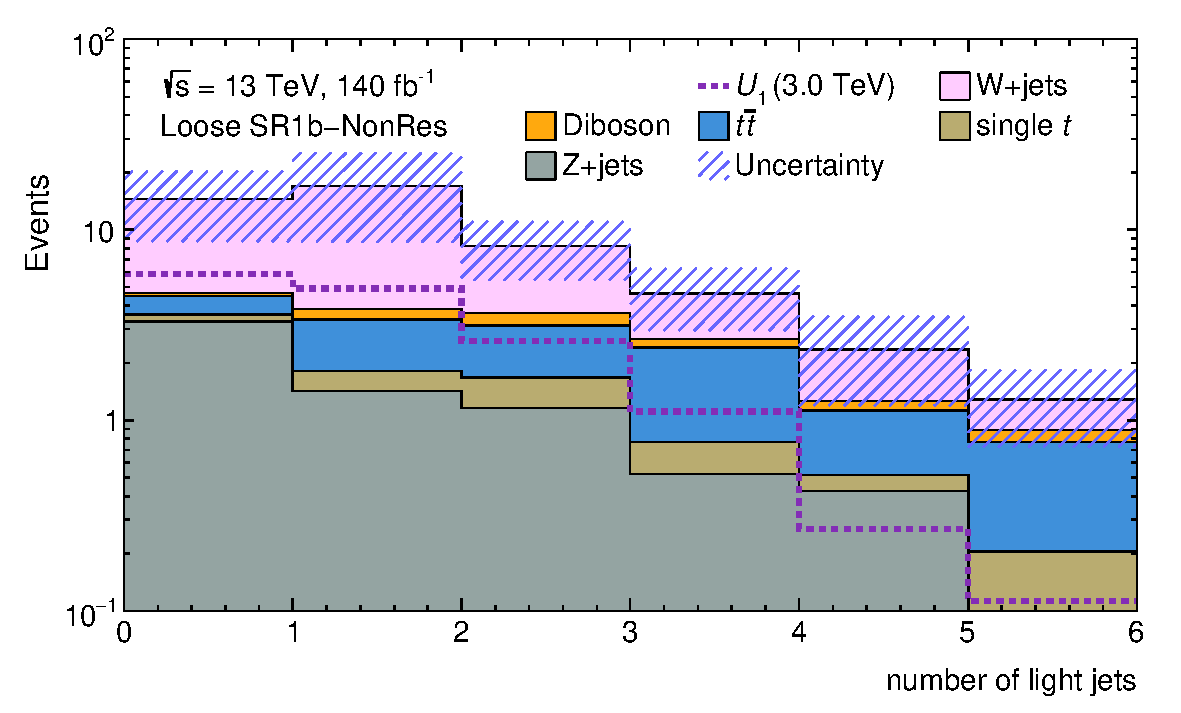
\includegraphics[width=\linewidth]{Figs/CH7/SR1b_NonRes_nlightjets.pdf}
        \caption{$N_j-N_b$.}
    \end{subfigure}\hfill
    \begin{subfigure}{0.49\linewidth}
        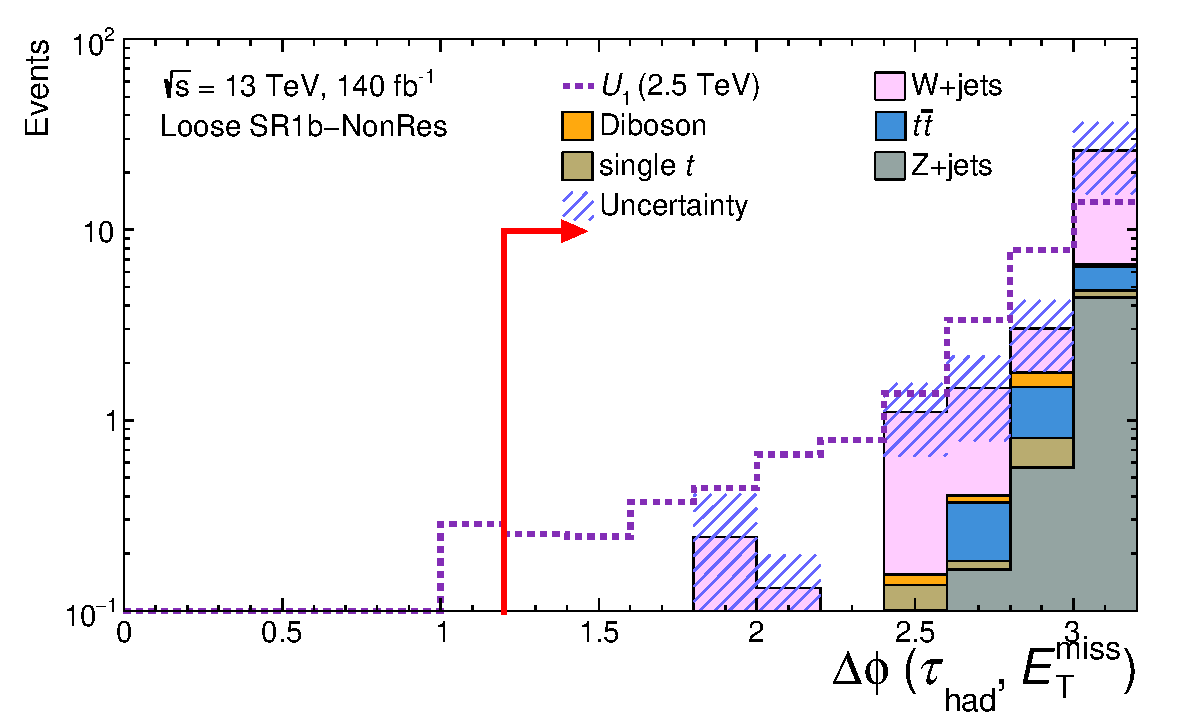
\includegraphics[width=\linewidth]{Figs/CH7/SR1b_NonRes_dphi.pdf}
        \caption{$\DphiTauMet$.}
    \end{subfigure}\par\medskip
    \caption[Loose N-1 distributions in SR1b-NonRes]{Distributions of the six scan variables in the loose non-resonant one-$b$-jet region. Before removing the plotted requirement, the thresholds are lowered to $\mT>500~\GeV$, $\met>300~\GeV$ and $\pT^\tau>100~\GeV$. The baseline $\met>200~\GeV$ is retained. The stacked backgrounds are shown before the fit, and the hatched band represents their uncertainty. The dotted signal curve is the pure BSM prediction at $(\MU,\gU,\beta_L^{23})=(3.0~\TeV,2.5,1.0)$.}
    \label{fig:ch7_sr1b_nonres_distributions}
\end{figure}

The remaining background in both one-$b$-jet regions is dominated by $W$+jets, principally $W\to\tau\nu$.
The tagged jet can originate from heavy-flavour production or a misidentified light-flavour jet.
In the final background prediction, after the control-region constraints described in Chapter~\ref{chapter:background_estimation}, $W$+jets contributes approximately $70\%$ in each region.
In $\bTagSR$-$\Res$, diboson production contributes about $15\%$, followed by $\ttbar$ and single-top production, including $Wt$.
In $\bTagSR$-$\NonRes$, $\ttbar$ contributes about $14\%$, $Z\to\tau\tau$+jets about $9\%$, and diboson production about $5\%$.
Top-quark events can pass the selection through $\ttbar\to b\tau\nu\,\bar b\tau\nu$ or $Wt\to b\tau\nu\,\tau\nu$ when only one $\tau$ is selected and the remaining decay products satisfy the jet and lepton requirements.
The $Z\to\tau\tau$ contribution similarly requires only one selected $\tau$, with neutrinos from the decays producing $\met$.
Among events with a jet misidentified as a $\tau$, $Z\to\nu\nu$+jets is the main source because the invisible $Z$ decay supplies genuine missing momentum.
Multijet production is negligible after the cleaning and full SR requirements.

\clearpage
\section[b-veto signal region definition (SR0b)]{b-veto signal region definition ($\bVetoSR$)}
\label{sec:ch7_sr0b}

The $\bVetoSR$ regions select signal events with no $b$-tagged jet and extend the sensitivity to large $\beta_L^{23}$.
As shown by the flavour current and coupling texture in Eqs.~\ref{eq:u1_current_expanded} and~\ref{eq:u1_beta_texture}, $\beta_L^{23}$ controls the $s\tau$ interaction and contributes $V_{cs}\beta_L^{23}$ to the $c\nu_\tau$ interaction.
The resulting zero-$b$-jet topologies were introduced in Section~\ref{subsec:lq_collider_benchmark}.
In particular, $U_1\to s\tau$ produces a resonant signal with a genuine non-$b$ jet, so $\bVetoSR$ retains a physically distinct signal contribution in addition to events in which a $b$-jet is not tagged or reconstructed.
The leading jet in $\bVetoSR$ is not explicitly identified as a strange-quark jet.
The truth-level study also identifies a substantial contribution with a leading $c$ jet.
At $(\MU,\gU,\beta_L^{23})=(1.5~\TeV,1.5,0.6)$, approximately $30\%$ and $60\%$ of the selected truth-level resonant-category events have a leading $s$ or $c$ jet, respectively.
The $s$-jet contribution contains the $s\tau$ resonance, whereas the $c$-jet contribution can contain an on-shell $U_1\to c\nu_\tau$ decay.
For the latter, the resonance is in the $c\nu_\tau$ system rather than the jet--$\tau$ system.
In the non-resonant truth-level category, approximately $33\%$ and $11\%$ of the events have a radiated leading $s$ or $c$ jet, with most of the remainder containing a gluon jet in $sc\to\tau\nu_\tau$ production.
These fractions describe the chosen benchmark and truth selection, rather than a flavour measurement of the reconstructed jets.

The two $\bVetoSR$ regions are defined by replacing the one-$b$-jet requirement with $N_b=0$ and using the leading jet in the topology-dependent selections.
The resonant region requires $\pT^{j_1}>250~\GeV$ and $m_{j\tau}>800~\GeV$, while the non-resonant region requires $50<\pT^{j_1}<250~\GeV$.
The $\pT^\tau$, $\met$, $\mT$ and $\DphiTauMet$ thresholds follow the corresponding one-$b$-jet regions.
The upper limits are imposed on the total jet multiplicity: $N_j\leq4$ for $\bVetoSR$-$\Res$ and $N_j\leq2$ for $\bVetoSR$-$\NonRes$.
These preserve the total jet limits used in $\bTagSR$ after replacing the tagged jet with an untagged leading jet.

The $\met>200~\GeV$ requirement in $\bVetoSR$-$\Res$ is retained to keep its kinematic selection aligned with $\bTagSR$-$\Res$.
A supplementary study of tighter $\met$ thresholds is presented in Appendix~\ref{app:sr0b_optimisation}.
The $\bVetoSR$-$\NonRes$ threshold remains $\met>400~\GeV$, which also maximises the significance in that study.

Signal efficiency in $\bVetoSR$ is evaluated for the pure BSM contribution, with $A\epsilon$ defined as in Section~\ref{subsec:ch7_efficiency}.
For illustration, at $(\MU,\gU,\beta_L^{23})=(1.5~\TeV,1.0,0.2)$ with $\beta_R^{33}=0$, $A\epsilon$ is $0.30\%$ and $0.13\%$ in $\bVetoSR$-$\Res$ and $\bVetoSR$-$\NonRes$, compared with $0.64\%$ and $0.069\%$ in the corresponding $\bTagSR$ regions.
These efficiencies depend on the mass and flavour couplings because the relative contributions of the production and decay channels change.
The destructive interference in the final zero-$b$-jet selections reduces the nominal pure BSM yield by approximately $20\%$ at $\MU=1.5~\TeV$ and by about $30$--$40\%$ at higher masses.
This reduction is appreciable even after the high-$\mT$ and $\met$ requirements, so the final prediction includes the signed interference contribution explicitly.
The supplementary $\met$ scan in Appendix~\ref{app:sr0b_optimisation} also shows that a higher $\met$ threshold can suppress this contribution.

Figure~\ref{fig:ch7_sr0b_distributions} shows the $m_{j\tau}$ distribution before the mass requirement in $\bVetoSR$-$\Res$.
It also shows the transverse-mass distribution above $600~\GeV$ in $\bVetoSR$-$\NonRes$.
The high-$m_{j\tau}$ requirement enhances the resonant signal contribution, while the high-$\mT$ requirement selects non-resonant production.
Together with the one-$b$-jet regions, these selections retain sensitivity to both $b\tau$ and $s\tau$ final states over the coupling range studied in this thesis.

\begin{figure}[htbp]
    \centering
    \begin{subfigure}{0.49\linewidth}
        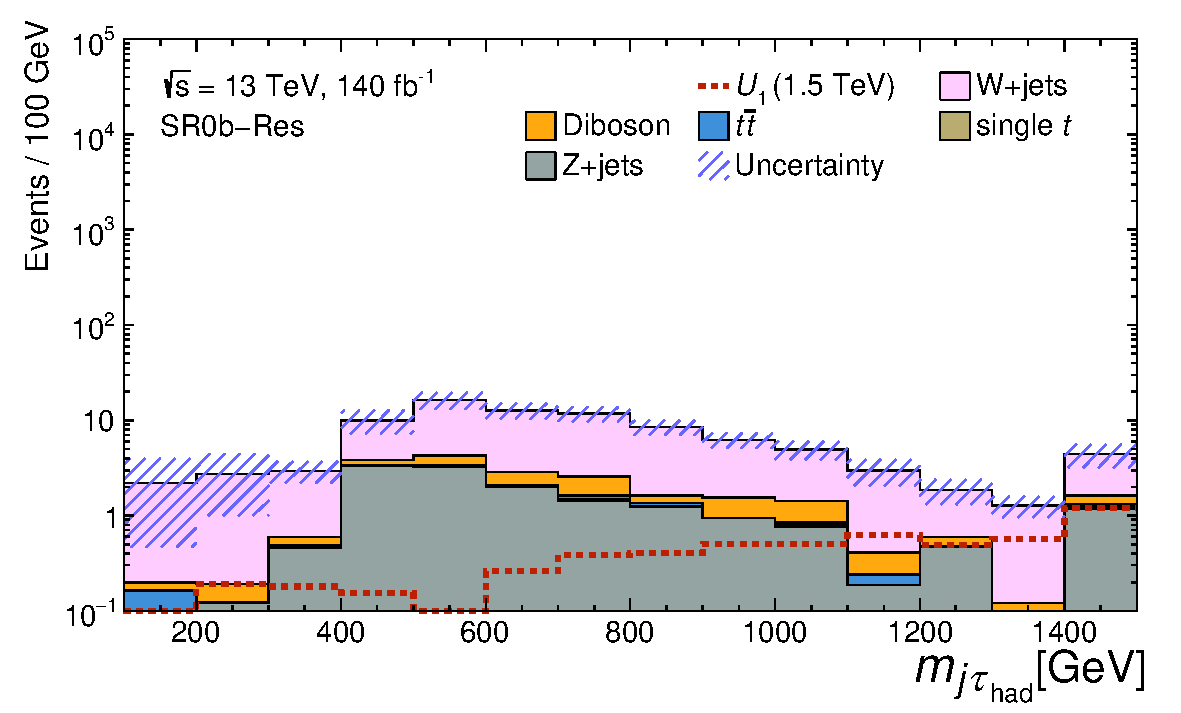
\includegraphics[width=\linewidth]{Figs/CH7/SR0b_Res_InvM.pdf}
        \caption{$\bVetoSR$-$\Res$: $m_{j\tau}$.}
    \end{subfigure}\hfill
    \begin{subfigure}{0.49\linewidth}
        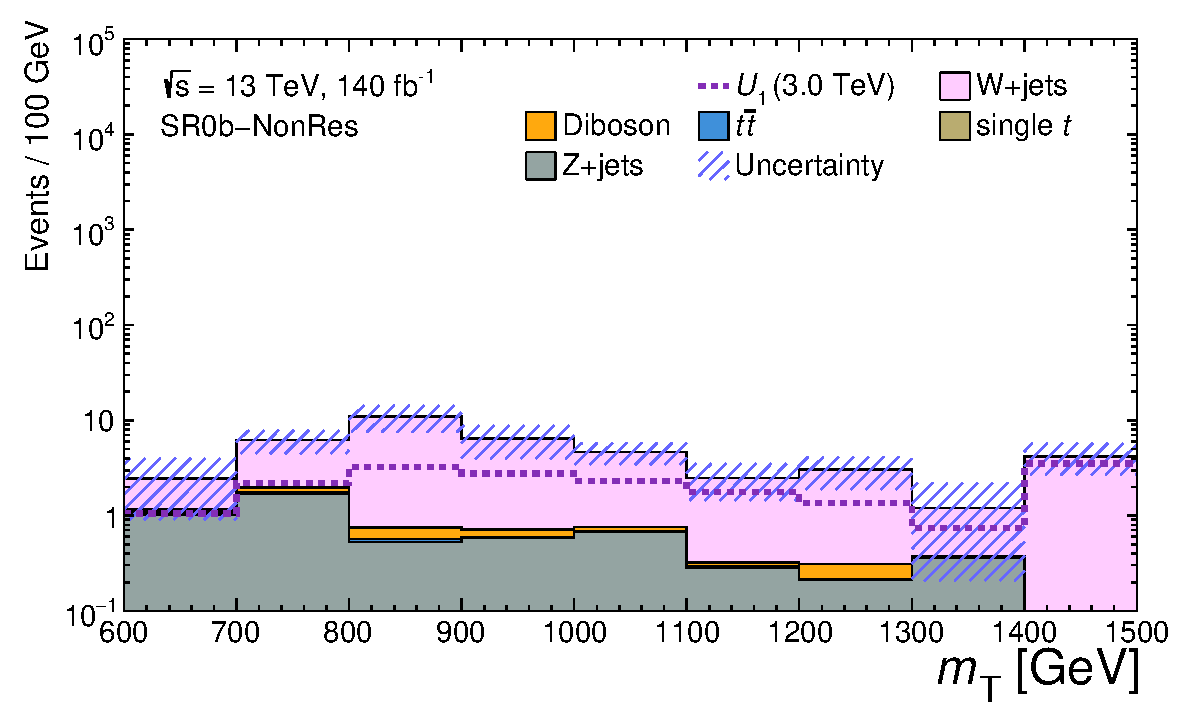
\includegraphics[width=\linewidth]{Figs/CH7/SR0b_NonRes_mT.pdf}
        \caption{$\bVetoSR$-$\NonRes$: $\mT$.}
    \end{subfigure}
    \caption[Discriminating-variable distributions in SR0b]{Distributions of (a) $m_{j\tau}$ in $\bVetoSR$-$\Res$ with the mass requirement removed and (b) $\mT$ in $\bVetoSR$-$\NonRes$ above $600~\GeV$. The other SR requirements are retained. The backgrounds are shown before the fit, and the hatched band represents their uncertainty. The dotted curves show pure BSM signals at $(\MU,\gU,\beta_L^{23})=(1.5~\TeV,1.5,0.6)$ in (a) and $(3.0~\TeV,2.5,1.0)$ in (b).}
    \label{fig:ch7_sr0b_distributions}
\end{figure}

The zero-$b$-jet background is dominated by $W\to\tau\nu$+jets, since vetoing tagged $b$ jets removes much of the top-quark background while retaining $W$ production with light-flavour jets.
In the final prediction after the control-region constraints, $W$+jets contributes approximately $76\%$ in $\bVetoSR$-$\Res$ and $82\%$ in $\bVetoSR$-$\NonRes$.
In the resonant region, diboson production contributes about $10\%$, $Z\to\nu\nu$+jets about $8\%$, and $Z\to\tau\tau$+jets about $5\%$.
In the non-resonant region, the corresponding contributions are approximately $3\%$, $6\%$ and $8\%$.
The $Z\to\nu\nu$ events contain a jet misidentified as a $\tau$, while $Z\to\tau\tau$ and diboson events can contain genuine $\tau$ leptons and neutrinos.
The combined $\ttbar$ and single-top contribution is below $1\%$ in each zero-$b$-jet region.

The final requirements for all four mutually exclusive SRs are summarised in Table~\ref{tab:ch7_signal_regions}.
Each region contributes one event count to the simultaneous statistical analysis.

\begin{table}[htbp]
    \centering
    \small
    \caption{Common baseline requirements and final signal-region selections. A dash denotes no additional requirement. The jet multiplicity includes $b$-tagged jets.}
    \label{tab:ch7_signal_regions}
    \begin{tabular}{lcccc}
        \toprule
        \multicolumn{5}{c}{Baseline requirements} \\
        \midrule
        Trigger & \multicolumn{4}{c}{Lowest-threshold unprescaled $\met$ trigger} \\
        $N_\tau$ & \multicolumn{4}{c}{1} \\
        $N_\ell=N_e+N_\mu$ & \multicolumn{4}{c}{0} \\
        Multijet suppression & \multicolumn{4}{c}{$\min\Delta\phi(j,\met)>0.4$ or $\met/\minDphiJetPt>6$} \\
        \midrule
        & \multicolumn{2}{c}{Resonant} & \multicolumn{2}{c}{Non-resonant} \\
        Requirement & $\bTagSR$-$\Res$ & $\bVetoSR$-$\Res$ & $\bTagSR$-$\NonRes$ & $\bVetoSR$-$\NonRes$ \\
        \midrule
        $N_b$ & 1 & 0 & 1 & 0 \\
        $\pT^b$ [$\GeV$] & $>250$ & -- & $50<\pT^b<250$ & -- \\
        $\pT^{j_1}$ [$\GeV$] & -- & $>250$ & -- & $50<\pT^{j_1}<250$ \\
        $\pT^\tau$ [$\GeV$] & \multicolumn{4}{c}{$>200$} \\
        $\met$ [$\GeV$] & \multicolumn{2}{c}{$>200$} & \multicolumn{2}{c}{$>400$} \\
        $\mT$ [$\GeV$] & \multicolumn{2}{c}{$>200$} & \multicolumn{2}{c}{$>600$} \\
        $m_{b\tau}$ [$\GeV$] & $>800$ & -- & -- & -- \\
        $m_{j\tau}$ [$\GeV$] & -- & $>800$ & -- & -- \\
        $\DphiTauMet$ & \multicolumn{2}{c}{--} & \multicolumn{2}{c}{$>1.2$} \\
        $N_j$ & \multicolumn{2}{c}{$\leq4$} & \multicolumn{2}{c}{$\leq2$} \\
        \bottomrule
    \end{tabular}
\end{table}

\clearpage
\section{Tau-pair signal contamination}
\label{sec:ch7_tautau_contamination}

Leptoquark production with a $\tau\tau$ final state can also populate the $\tau\nu+\mathrm{jets}$ signal regions.
Although two $\tau$-leptons are produced, an event can satisfy the single-$\tau$ requirement when only one is reconstructed and selected.
Neutrinos from the $\tau$ decays produce missing momentum.
This is an additional BSM contribution from the same $U_1$ model, rather than an SM background.

The study uses simulated $\tau\tau$ samples generated with $\beta_L^{33}=1$, $\beta_R^{33}=0$ and $\beta_L^{23}=0$.
Their selected yields are compared with available $\tau\nu$ samples near the exclusion sensitivity, at $(\MU,\gU,\beta_L^{23})=(1.8~\TeV,3.0,0.6)$ and $(3.0~\TeV,2.0,1.4)$.
The corresponding $\tau\tau$ samples use $\gU=2.8$ and $2.1$.
The $\tau\tau$ production cross section is recalculated with \textsc{MadGraph5\_aMC@NLO} at larger $\beta_L^{23}$, and the selected yields are scaled by the cross-section ratio to their generation point.
This estimates the additional rate while retaining the acceptance and kinematic shapes of the available samples.
It therefore provides a sensitivity study rather than a simulation of the full coupling dependence of the $\tau\tau$ acceptance.

The estimated additional yield is of order $35\%$ of the nominal $\tau\nu$ yield in the one-$b$-jet regions and several percent in the zero-$b$-jet regions.
To assess the effect on the search, the nominal signal predictions are increased by the factors shown in Table~\ref{tab:ch7_tautau_contamination}, and the exclusion fit is repeated.

\begin{table}[htbp]
    \centering
    \caption{Additional signal normalisation used to estimate the sensitivity to $\tau\tau$ production. The factors multiply the nominal $\tau\nu$ signal prediction in the supplementary fit.}
    \label{tab:ch7_tautau_contamination}
    \begin{tabular}{lcc}
        \toprule
        Region & Additional contribution & Applied factor \\
        \midrule
        $\bTagSR$-$\Res$ & $37\%$ & 1.37 \\
        $\bTagSR$-$\NonRes$ & $33\%$ & 1.33 \\
        $\bVetoSR$-$\Res$ & $5\%$ & 1.05 \\
        $\bVetoSR$-$\NonRes$ & $7\%$ & 1.07 \\
        \bottomrule
    \end{tabular}
\end{table}

The expected upper limit on the signal strength improves by approximately $8$--$14\%$ in this test.
The corresponding change in the coupling limit is smaller because the signal rate depends strongly on $\gU$.
At $\MU=1.8~\TeV$ and $\beta_L^{23}=0.6$, the expected upper limit on $\gU$ changes from 2.18 to 2.07, an improvement of approximately $5\%$.
At $\MU=3.0~\TeV$ and $\beta_L^{23}=1.4$, it changes from 1.96 to 1.91, or approximately $2.6\%$.
The nominal interpretation retains the $\tau\nu$ signal model.
The supplementary study indicates that the omitted positive $\tau\tau$ contribution could strengthen the expected coupling constraints by a few percent under the assumptions used for the rate estimate.
